%%
%% This is file `sample-sigconf-authordraft.tex',
%% generated with the docstrip utility.
%%
%% The original source files were:
%%
%% samples.dtx  (with options: `all,proceedings,bibtex,authordraft')
%% 
%% IMPORTANT NOTICE:
%% 
%% For the copyright see the source file.
%% 
%% Any modified versions of this file must be renamed
%% with new filenames distinct from sample-sigconf-authordraft.tex.
%% 
%% For distribution of the original source see the terms
%% for copying and modification in the file samples.dtx.
%% 
%% This generated file may be distributed as long as the
%% original source files, as listed above, are part of the
%% same distribution. (The sources need not necessarily be
%% in the same archive or directory.)
%%
%%
%% Commands for TeXCount
%TC:macro \cite [option:text,text]
%TC:macro \citep [option:text,text]
%TC:macro \citet [option:text,text]
%TC:envir table 0 1
%TC:envir table* 0 1
%TC:envir tabular [ignore] word
%TC:envir displaymath 0 word
%TC:envir math 0 word
%TC:envir comment 0 0
%%
%% The first command in your LaTeX source must be the \documentclass
%% command.
%%
%% For submission and review of your manuscript please change the
%% command to \documentclass[manuscript, screen, review]{acmart}.
%%
%% When submitting camera ready or to TAPS, please change the command
%% to \documentclass[sigconf]{acmart} or whichever template is required
%% for your publication.
%%
%%
\PassOptionsToPackage{table}{xcolor}
\documentclass[sigconf,authordraft]{acmart}
%%
%% \BibTeX command to typeset BibTeX logo in the docs
\AtBeginDocument{%
  \providecommand\BibTeX{{%
    Bib\TeX}}}

%% Rights management information.  This information is sent to you
%% when you complete the rights form.  These commands have SAMPLE
%% values in them; it is your responsibility as an author to replace
%% the commands and values with those provided to you when you
%% complete the rights form.
\setcopyright{acmlicensed}
\copyrightyear{2018}
\acmYear{2018}
\acmDOI{XXXXXXX.XXXXXXX}
%% These commands are for a PROCEEDINGS abstract or paper.
\acmConference[Conference acronym 'XX]{Make sure to enter the correct
  conference title from your rights confirmation email}{June 03--05,
  2018}{Woodstock, NY}
%%
%%  Uncomment \acmBooktitle if the title of the proceedings is different
%%  from ``Proceedings of ...''!
%%
%%\acmBooktitle{Woodstock '18: ACM Symposium on Neural Gaze Detection,
%%  June 03--05, 2018, Woodstock, NY}
\acmISBN{978-1-4503-XXXX-X/2018/06}


%%
%% Submission ID.
%% Use this when submitting an article to a sponsored event. You'll
%% receive a unique submission ID from the organizers
%% of the event, and this ID should be used as the parameter to this command.
%%\acmSubmissionID{123-A56-BU3}

%%
%% For managing citations, it is recommended to use bibliography
%% files in BibTeX format.
%%
%% You can then either use BibTeX with the ACM-Reference-Format style,
%% or BibLaTeX with the acmnumeric or acmauthoryear sytles, that include
%% support for advanced citation of software artefact from the
%% biblatex-software package, also separately available on CTAN.
%%
%% Look at the sample-*-biblatex.tex files for templates showcasing
%% the biblatex styles.
%%

%%
%% The majority of ACM publications use numbered citations and
%% references.  The command \citestyle{authoryear} switches to the
%% "author year" style.
%%
%% If you are preparing content for an event
%% sponsored by ACM SIGGRAPH, you must use the "author year" style of
%% citations and references.
%% Uncommenting
%% the next command will enable that style.
%%\citestyle{acmauthoryear}

\usepackage{xspace}
% \usepackage{xcolor}
\usepackage{graphicx} 
\usepackage{caption}
\usepackage{subcaption}
% \usepackage{hyperref}
\usepackage{cleveref}
\usepackage{multirow}
\usepackage[inline]{enumitem}
\usepackage{booktabs}
\usepackage{array}
\usepackage{pifont}

% xcolor with table option is now loaded via \PassOptionsToPackage before \documentclass
\usepackage{makecell}
\newcolumntype{M}[1]{>{\centering\arraybackslash}m{#1}}

\newcommand{\sysname}{Cygnus\xspace}
\newcommand{\libos}{\texttt{libCyg}\xspace}
\newcommand{\schedcore}{\textsc{Deneb}\xspace}
\newcommand{\kmod}{\textsc{KActiv}\xspace}
\newcommand{\yihan}[1]{\textcolor{orange}{yihan:#1}\xspace}

%%
%% end of the preamble, start of the body of the document source.
\begin{document}

%%
%% The "title" command has an optional parameter,
%% allowing the author to define a "short title" to be used in page headers.
\title{\sysname}

%%
%% The "author" command and its associated commands are used to define
%% the authors and their affiliations.
%% Of note is the shared affiliation of the first two authors, and the
%% "authornote" and "authornotemark" commands
%% used to denote shared contribution to the research.
% \author{Yihan Yang}
% \email{}
% \orcid{}
% \author{}
% \authornotemark[1]
% \email{}
% \affiliation{%
%   \institution{National University of Singapore}
%   \city{Singapore}
%   \country{Singapore}
% }

%%
%% By default, the full list of authors will be used in the page
%% headers. Often, this list is too long, and will overlap
%% other information printed in the page headers. This command allows
%% the author to define a more concise list
%% of authors' names for this purpose.
\renewcommand{\shortauthors}{Trovato et al.}

%%
%% The abstract is a short summary of the work to be presented in the
%% article.
\begin{abstract}
  A clear and well-documented \LaTeX\ document is presented as an
  article formatted for publication by ACM in a conference proceedings
  or journal publication. Based on the ``acmart'' document class, this
  article presents and explains many of the common variations, as well
  as many of the formatting elements an author may use in the
  preparation of the documentation of their work.
\end{abstract}

%%
%% The code below is generated by the tool at http://dl.acm.org/ccs.cfm.
%% Please copy and paste the code instead of the example below.
%%
\begin{CCSXML}
<ccs2012>
 <concept>
  <concept_id>00000000.0000000.0000000</concept_id>
  <concept_desc>Do Not Use This Code, Generate the Correct Terms for Your Paper</concept_desc>
  <concept_significance>500</concept_significance>
 </concept>
 <concept>
  <concept_id>00000000.00000000.00000000</concept_id>
  <concept_desc>Do Not Use This Code, Generate the Correct Terms for Your Paper</concept_desc>
  <concept_significance>300</concept_significance>
 </concept>
 <concept>
  <concept_id>00000000.00000000.00000000</concept_id>
  <concept_desc>Do Not Use This Code, Generate the Correct Terms for Your Paper</concept_desc>
  <concept_significance>100</concept_significance>
 </concept>
 <concept>
  <concept_id>00000000.00000000.00000000</concept_id>
  <concept_desc>Do Not Use This Code, Generate the Correct Terms for Your Paper</concept_desc>
  <concept_significance>100</concept_significance>
 </concept>
</ccs2012>
\end{CCSXML}

\ccsdesc[500]{Do Not Use This Code~Generate the Correct Terms for Your Paper}
\ccsdesc[300]{Do Not Use This Code~Generate the Correct Terms for Your Paper}
\ccsdesc{Do Not Use This Code~Generate the Correct Terms for Your Paper}
\ccsdesc[100]{Do Not Use This Code~Generate the Correct Terms for Your Paper}

%%
%% Keywords. The author(s) should pick words that accurately describe
%% the work being presented. Separate the keywords with commas.
\keywords{Do, Not, Use, This, Code, Put, the, Correct, Terms, for,
  Your, Paper}
%% A "teaser" image appears between the author and affiliation
%% information and the body of the document, and typically spans the
%% page.
% \begin{teaserfigure}
%   \includegraphics[width=\textwidth]{sampleteaser}
%   \caption{Seattle Mariners at Spring Training, 2010.}
%   \Description{Enjoying the baseball game from the third-base
%   seats. Ichiro Suzuki preparing to bat.}
%   \label{fig:teaser}
% \end{teaserfigure}

\received{20 February 2007}
\received[revised]{12 March 2009}
\received[accepted]{5 June 2009}

%%
%% This command processes the author and affiliation and title
%% information and builds the first part of the formatted document.
\maketitle

\section{Introduction}
\label{sec:intro}
Modern datacenter applications operate under strict microsecond-scale Service Level Objectives (SLOs) while exhibiting distinct workload characteristics. 
These workloads differ in request arrival patterns and service time distributions.
For example, microservice often experiences high request dispersion while serverless platforms and financial trading systems often exhibit more uniform workloads yet bursty traffic patterns.

The diversity in application workloads motivates the need for tailoring scheduling policies to meet specific SLOs.
Tail latency-sensitive services, such as in-memory key-value stores and web search, benefit from preemptive scheduling to minimize queueing delays. 
In contrast, interactive applications like e-commerce and social media prioritize responsiveness, often requiring policies like Shortest Remaining Processing Time (SRPT) to minimize mean latency.
Moreover, soft real-time workloads, including video conferencing and online gaming, operate under strict temporal constraints, demanding deadline-aware scheduling to guarantee frame rates and minimize jitter.

However, enforcing application-specific scheduling policies at microsecond-scale remains to be challenging.
Traditional kernel schedulers provide abundant scheduling policies but operate at millisecond timescales, unsuitable for modern applications.
To compensate, recent dataplane operating systems (OSes) bypass the kernel to achieve microsecond-scale preemptive scheduling in userspace.
Yet they lack the flexibility for applications to define custom scheduling policies.
Instead, they rigidly hardcode a hybrid policy by combining centralized First-Come-First-Served (FCFS) for light-tailed workloads with Processor Sharing (PS) for heavy-tailed workloads.

In this paper, we present the design of \kernel, a datapath OS that extends the Exokernel philosophy to hardware interrupt control.
Our key insight is that direct userspace access to system-critical interrupt hardware is the missing piece to achieving kernel-level scheduling flexibility in current dataplane OSes.
Therefore, the goal of \kernel is to redefine the OS-application boundary to safely expose these interrupts into userspace, thereby enabling applications to build custom scheduling policies directly around these low-level events.

\kernel relies on three key techniques to unite the policy flexibility of kernel schedulers with the microsecond-scale performance of dataplane OSes.
First, \kernel provides a scheduling core abstraction that enables applications to implement custom scheduling policies with kernel events in userspace.
Second, \kernel introduces a lightweight isolation mechanism that securely exposes low-level interrupt hardware to untrusted userspace components with minimal overhead.
Third, \kernel introduces a hardware multiplexing mechanism that safely shares system-critical resources (e.g., LAPIC timer) among multiple untrusted userspace schedulers.

\section{Motivation}
\label{sec:motivation}
In this section, we analyze the scalability challenges inherent in centralized preemption architectures. 
We first profile the overhead of preemption mechanisms commonly used in existing dataplane OSes, including POSIX signals, Inter-Processor Interrupts (IPIs), and cache-coherent messaging (\S~\ref{subsec:profiling-preemption-mechanisms}).
Based on these empirical measurements, we construct an analytical model to formalize the scalability limits of a centralized dispatcher (\S~\ref{subsec:model-setup}).
We then use the model to evaluate how increasing the core count impacts system performance across three key dimensions: total preemption overhead (\S~\ref{subsec:preemption-overhead}), preemption precision drift (\S~\ref{subsec:preemption-precision-drift}), as well as core efficiency and throughput loss (\S~\ref{subsec:core-efficiency-and-throughput-loss}).

\subsection{Profiling Common Preemption Mechanisms}
\label{subsec:profiling-preemption-mechanisms}

\subsection{Model Setup}
\label{subsec:model-setup}

We consider a system with $N$ cores in total.
% Out of these, $n_w$ cores are available for worker threads, while $n_d$ cores are dedicated to preemption dispatching.
% Thus, we have the constraint that $N = n_w + n_d$.
% We define preemption quantum $q$.
% We first consider the case where the dispatcher uses a single core, i.e., $n_d = 1$.
% We later extend the model to consider multiple dispatcher cores for core efficiency analysis.

\subsection{Preemption Overhead}
\label{subsec:preemption-overhead}

\subsection{Preemption Precision Drift}
\label{subsec:preemption-precision-drift}

\subsection{Core Efficiency and Throughput Loss}
\label{subsec:core-efficiency-and-throughput-loss}

% We now analyze the scalability challenges of using a centralized dispatcher to preempt worker cores:
% as core counts grow, the overhead of issuing preemptions increases, forcing a
% trade-off between preemption precision and core efficiency.
% This trade-off can be illustrated by two extreme dispatching policies:
% \begin{enumerate*}[label=(\roman*)]
%   \item \textit{Sequential unicast}, where the dispatcher preempts individual cores one at a time using unicast IPIs, and
%   \item \textit{Batched multicast}, where the dispatcher preempts all cores at once using multicast IPIs
% \end{enumerate*}.
% Sequential unicast policy enables precise per-core control over preemption timing, allowing each worker to be preempted exactly when needed.
% However, this approach requires the dispatcher to track and interrupt each core independently, incurring overhead that grows linearly with the number of cores.
% In contrast, batched multicast mitigates this overhead by sending a single interrupt to multiple cores at once, yet the cost still grows linearly to the number of batched cores(\cref{preemption-in-dataplane-os}) and worker cores must wait for the next batch to be preempted.
% The policy design space is infinite, but essentially trades off preemption precision against preemption overhead between these two extremes.
% To prove this, we also have a \textit{partial batching policy}, where the dispatcher issues preemptions to groups of worker cores via multicast IPIs.

% We use an analytical model to illustrate the scalability dilemma of centralized preemption dispatchers.

% \paragraph{System setup}
% We consider a system with $N$ cores in total.
% Out of these, $n_w$ cores are available for worker threads, while $n_d$ cores are dedicated to preemption dispatching.
% Thus, we have the constraint that $N = n_w + n_d$.
% We define preemption quantum $q$.
% We first consider the case where the dispatcher uses a single core, i.e., $n_d = 1$.
% We later extend the model to consider multiple dispatcher cores for core efficiency analysis.

% We define \textit{preemption drift} $\delta_i$ as the difference between the ideal preemption time (preemption quantum $q$) and actual preemption time when the preemption is received by core $i$.
% The worst-case preemption drift across all cores is defined as $\Delta = \max_{i=1}^{n_w} \delta_i$.
% Based on the profiling result in \cref{preemption-in-dataplane-os}, we define the cost of sending unicast IPI as $c_u$ and multicast IPI as the sum of base cost $c_b$ and incremental cost per core $c_m$:
% \begin{equation}
% C_{\text{multi}}(n) = c_b + n \cdot c_m
% \end{equation}

% \paragraph{Preemption overhead}

% We now analyze the dispatcher utilization for each policy.
% Workers at full capacity generate preemption events at rate $f/q$ per worker (where $f$ is the CPU frequency), yielding a system-wide preemption rate of $n_w \cdot f/q$.

% \textbf{Sequential unicast.}
% The dispatcher sends $n_w$ unicast IPIs per quantum, consuming $n_w \cdot c_u$ cycles.
% Dispatcher utilization is:
% \begin{equation}
% \rho_{\text{seq}} = \frac{n_w \cdot c_u}{q}
% \label{eq:util-seq}
% \end{equation}

% \textbf{Batched multicast.}
% The dispatcher sends one multicast IPI to all $n_w$ workers per quantum, consuming $C_{\text{multi}}(n_w)$ cycles.
% Dispatcher utilization is:
% \begin{equation}
% \rho_{\text{batch}} = \frac{c_b + n_w \cdot c_m}{q}
% \label{eq:util-batch}
% \end{equation}

% \textbf{Partial batching.}
% The dispatcher sends $g$ multicast IPIs per quantum, each to a group of $\lceil n_w / g \rceil$ workers.
% Dispatcher utilization is:
% \begin{equation}
% \rho_{\text{partial}}(g) = \frac{g \cdot c_b + n_w \cdot c_m}{q}
% \label{eq:util-partial}
% \end{equation}

% For stability, we require $\rho < 1$.
% This yields maximum scalable workers:
% \begin{align}
% {n_w}^{\text{max}}_{\text{seq}} &= \left\lfloor \frac{q}{c_u} \right\rfloor \\
% {n_w}^{\text{max}}_{\text{batch}} &= \left\lfloor \frac{q - c_b}{c_m} \right\rfloor
% \end{align}

% Since $c_u > c_m$ (unicast is more expensive than incremental multicast cost), batched multicast can support more workers with a single dispatcher.
% However, both policies exhibit \textit{linear} growth in dispatcher utilization with $n_w$, as shown in \Cref{fig:overhead-scaling}.

% \begin{figure}[t]
%   \centering
%   \includegraphics[width=0.8\columnwidth]{figs/overhead-scaling.pdf}
%   \caption{Dispatcher utilization versus number of worker cores. Both sequential and batched policies exhibit linear growth, but batched has a smaller slope ($c_m < c_u$).}
%   \label{fig:overhead-scaling}
% \end{figure}

% \paragraph{Preemption precision drift}

% We analyze precision drift for each policy assuming all workers reach their quantum boundary simultaneously in the worst case.

% \textbf{Sequential unicast.}
% A single dispatcher ($n_d = 1$) monitors all $n_w$ workers.
% When a worker reaches quantum $q$, the dispatcher sends a unicast IPI with cost $c_u$.
% In the worst case, all workers reach their quantum at the same ideal time $t_0$, and the dispatcher processes them sequentially:
% worker $i$ receives its preemption IPI at time $t_0 + (i-1) \cdot c_u$, yielding drift $\delta_i = (i-1) \cdot c_u$.

% The worst-case preemption drift is:
% \begin{equation}
% \Delta_{\text{seq}} = c_u \cdot (n_w - 1)
% \label{eq:drift-seq}
% \end{equation}

% \textbf{Batched multicast.}
% A single dispatcher sends periodic multicast IPIs to all $n_w$ workers at fixed intervals equal to the quantum $q$.
% Batches are sent at times $0, q, 2q, \ldots$.
% A worker reaching its quantum at time $t = kq + \tau$ (where $\tau \in [0, q)$) must wait until the next batch at $(k+1)q$, incurring drift $\delta = q - \tau$.

% The worst-case preemption drift is:
% \begin{equation}
% \Delta_{\text{batch}} = q
% \label{eq:drift-batch}
% \end{equation}

% \textbf{Partial batching.}
% We introduce an intermediate policy parameterized by the number of groups $g$ ($1 \leq g \leq n_w$).
% The dispatcher partitions workers into $g$ groups, each with $\lceil n_w / g \rceil$ workers.
% At each quantum boundary, the dispatcher sequentially sends multicast IPIs to each group.
% Workers in group $j$ experience drift from both batch alignment (waiting for the quantum boundary) and sequential group processing:
% \begin{equation}
% \delta_j = q + (j-1) \cdot C_{\text{multi}}\left(\left\lceil \frac{n_w}{g} \right\rceil\right)
% \end{equation}

% The worst-case drift is:
% \begin{equation}
% \Delta_{\text{partial}}(g) = q + (g-1) \left( c_b + \left\lceil \frac{n_w}{g} \right\rceil \cdot c_m \right)
% \label{eq:drift-partial}
% \end{equation}

% This interpolates between the two extremes:
% for $g = 1$ (fully batched), $\Delta_{\text{partial}}(1) = q = \Delta_{\text{batch}}$;
% for $g = n_w$ with $c_u = c_b + c_m$ (fully sequential), $\Delta_{\text{partial}}(n_w) = q + (n_w-1)c_u$.

% \textbf{Key observation.}
% Sequential unicast drift grows \textit{linearly} with worker count ($\Delta_{\text{seq}} \propto n_w$), while batched multicast drift remains \textit{constant} but equals the full quantum ($\Delta_{\text{batch}} = q$).
% \Cref{fig:drift-scaling} illustrates this fundamental trade-off.

% \begin{figure}[t]
%   \centering
%   \includegraphics[width=0.8\columnwidth]{figs/drift-scaling.pdf}
%   \caption{Worst-case preemption drift versus number of worker cores for different policies. Sequential drift grows linearly with $n_w$, while batched drift remains constant at $q$.}
%   \label{fig:drift-scaling}
% \end{figure}

% \paragraph{Core efficiency}

% To maintain system stability while scaling to large core counts, we can dedicate multiple cores to dispatching ($n_d > 1$).
% With $n_d$ dispatchers, each handles $\lceil n_w / n_d \rceil$ workers.

% \textbf{Sequential with multiple dispatchers.}
% Each dispatcher sends $\lceil n_w / n_d \rceil$ unicast IPIs per quantum.
% For stability, we require:
% \begin{equation}
% n_d \geq \left\lceil \frac{n_w \cdot c_u}{q} \right\rceil
% \label{eq:dispatchers-seq}
% \end{equation}

% With multiple dispatchers, precision drift improves:
% \begin{equation}
% \Delta_{\text{seq}}(n_d) = c_u \left( \left\lceil \frac{n_w}{n_d} \right\rceil - 1 \right)
% \label{eq:drift-seq-multi}
% \end{equation}

% \textbf{Batched with multiple dispatchers.}
% Workers are partitioned into $n_d$ groups, each served by one dispatcher sending multicast IPIs.
% For stability:
% \begin{equation}
% n_d \geq \left\lceil \frac{n_w \cdot c_m}{q} \right\rceil
% \label{eq:dispatchers-batch}
% \end{equation}

% However, precision drift remains unchanged:
% \begin{equation}
% \Delta_{\text{batch}}(n_d) = q
% \end{equation}

% Adding dispatchers reduces overhead but does not improve precision for batched policies.

% \textbf{Worker efficiency.}
% Given the constraint $N = n_w + n_d$, the fraction of cores available for useful work is $\eta = n_w / N$.
% Substituting the stability requirements:

% For sequential:
% \begin{equation}
% \eta_{\text{seq}} = \frac{n_w}{N} \leq \frac{q}{q + c_u}
% \label{eq:efficiency-seq}
% \end{equation}

% For batched:
% \begin{equation}
% \eta_{\text{batch}} = \frac{n_w}{N} \leq \frac{q}{q + c_m}
% \label{eq:efficiency-batch}
% \end{equation}

% Since $c_m < c_u$, batched achieves higher worker efficiency.
% However, as $N \to \infty$, both policies lose a \textit{constant fraction} of cores to dispatching: sequential loses $c_u/(q+c_u)$ and batched loses $c_m/(q+c_m)$.

% \Cref{fig:efficiency-tradeoff} illustrates the fundamental trade-off: sequential can trade dispatcher cores for better precision (by increasing $n_d$), while batched achieves better efficiency but cannot improve precision regardless of $n_d$.

% \begin{figure}[t]
%   \centering
%   \includegraphics[width=0.8\columnwidth]{figs/efficiency-tradeoff.pdf}
%   \caption{Worker efficiency versus worst-case drift for different policies and dispatcher allocations. Sequential policies can trade efficiency for precision, while batched policies achieve higher efficiency but are bounded by drift = $q$.}
%   \label{fig:efficiency-tradeoff}
% \end{figure}

% \textbf{Fundamental limit.}
% Our model reveals a fundamental scalability dilemma for centralized preemption dispatchers: achieving tight precision ($\Delta \ll q$) requires sacrificing core efficiency (dedicating $\Theta(n_w)$ dispatcher cores), while maintaining high efficiency ($\eta \approx 1$) results in poor precision ($\Delta = \Theta(q)$ or worse).
% No centralized architecture can simultaneously achieve constant precision, constant dispatcher overhead, and unbounded scalability.
% This motivates our design of a decentralized preemption mechanism in \Cref{sec:design}.


\section{Background}
\label{sec:background}
\subsection{Existing Uses of Preemption in Dataplane OS}

State-of-the-art dataplane OS schedulers use preemptive scheduling to reduce the impact of head-of-line blocking on tail latency.
Preemption can appear on both control path and datapath.

\paragraph{Control path preemption.}
Scheduler balances load across cores or adjusts core allocation for applications. 
This aims to maintain low core utilization to indirectly avoid head-of-line blocking and reduce queuing delays.
This type of preemption have more relaxed timing requirements since it does not directly affect latency-critical tasks.

\paragraph{Data path preemption.}
Scheduler directly preempts running tasks on the latency-critical datapath.
This aims to approximate Processor Sharing.
This type of preemption requires precise timing to ensure latency-sensitive tasks receive timely execution and low overhead to avoid excessive disruption to the datapath.

Existing works explore various preemption mechanisms, including POSIX signals, Inter-Processor Interrupts (IPIs), and cache-coherent message passing.
\yihan{We compare the overhead of these mechanisms in table xx.}

\subsection{Scalability Dilemma of Centralized Preemption}

We now discuss the scalability challenges of using a centralized preemption dispatcher to preempt remote worker cores.

Centralized preemption dispatcher implementation spectrum has two extremes:
\begin{enumerate*}[label=(\roman*)]
  \item \textit{Per-core preemption}, where the dispatcher issues preemptions to individual cores immediately to ensure precise preemption, and
  \item \textit{Batch-all preemption}, where the dispatcher issues preemptions to all cores at fixed intervals to minimize preemption issuing overhead.
\end{enumerate*}
\yihan{Explain why intermediate designs are bounded by these two}

We use an analytical model to illustrate the scalability dilemma of centralized preemption dispatchers.

\paragraph{System setup}
We consider a system with $n$ worker cores and preemption quantum $q$.
We define \textit{preemption drift} $\delta_i$ as the difference between the ideal preemption time (preemption quantum $q$) and actual preemption time when the preemption is received by core $i$.
The worst-case preemption drift across all cores is defined as $\Delta = \max_{i=1}^{n} \delta_i$.

% \paragraph{Preemption precision and preemption overhead}
% Centralized dispatchers face a fundamental trade-off between preemption precision and preemption overhead.
% In the instant per-core preemption extreme, the dispatcher issues preemptions to each core immediately.
% This ensures high preemption precision of $O(1)$, but incurs preemption overhead of $O(n)$, since the dispatcher must issue preemptions to all $n$ cores individually.
% In contrast, in the fixed-interval batch-all preemption extreme, the dispatcher issues preemptions to all cores at fixed intervals.
% This minimizes preemption overhead to $O(1)$, but results in low preemption precision of $O(q)$, since a core may have to wait up to $q$ time before receiving a preemption.

% \paragraph{Preemption precision and core efficiency}

\subsection{Hardware Isolation}

\section{Challenges and Approaches}
\label{sec:challenge}
Our goal is to design a dataplane OS that can perform scalable, microsecond-scale preemptive scheduling on modern multi-core servers.
To achieve this, we need to multiplex kernel-critical hardware resources like the LAPIC timer to a userspace scheduler without compromising system safety.
We need to address two key challenges:
\paragraph{Multiplexing hardware between the kernel and userspace}
\paragraph{Fast hardware configuration and secure event delivery}

\subsection{\sysname Approach}

\section{\sysname Design}
\label{sec:design}
\subsection{Overview}

\begin{figure}
    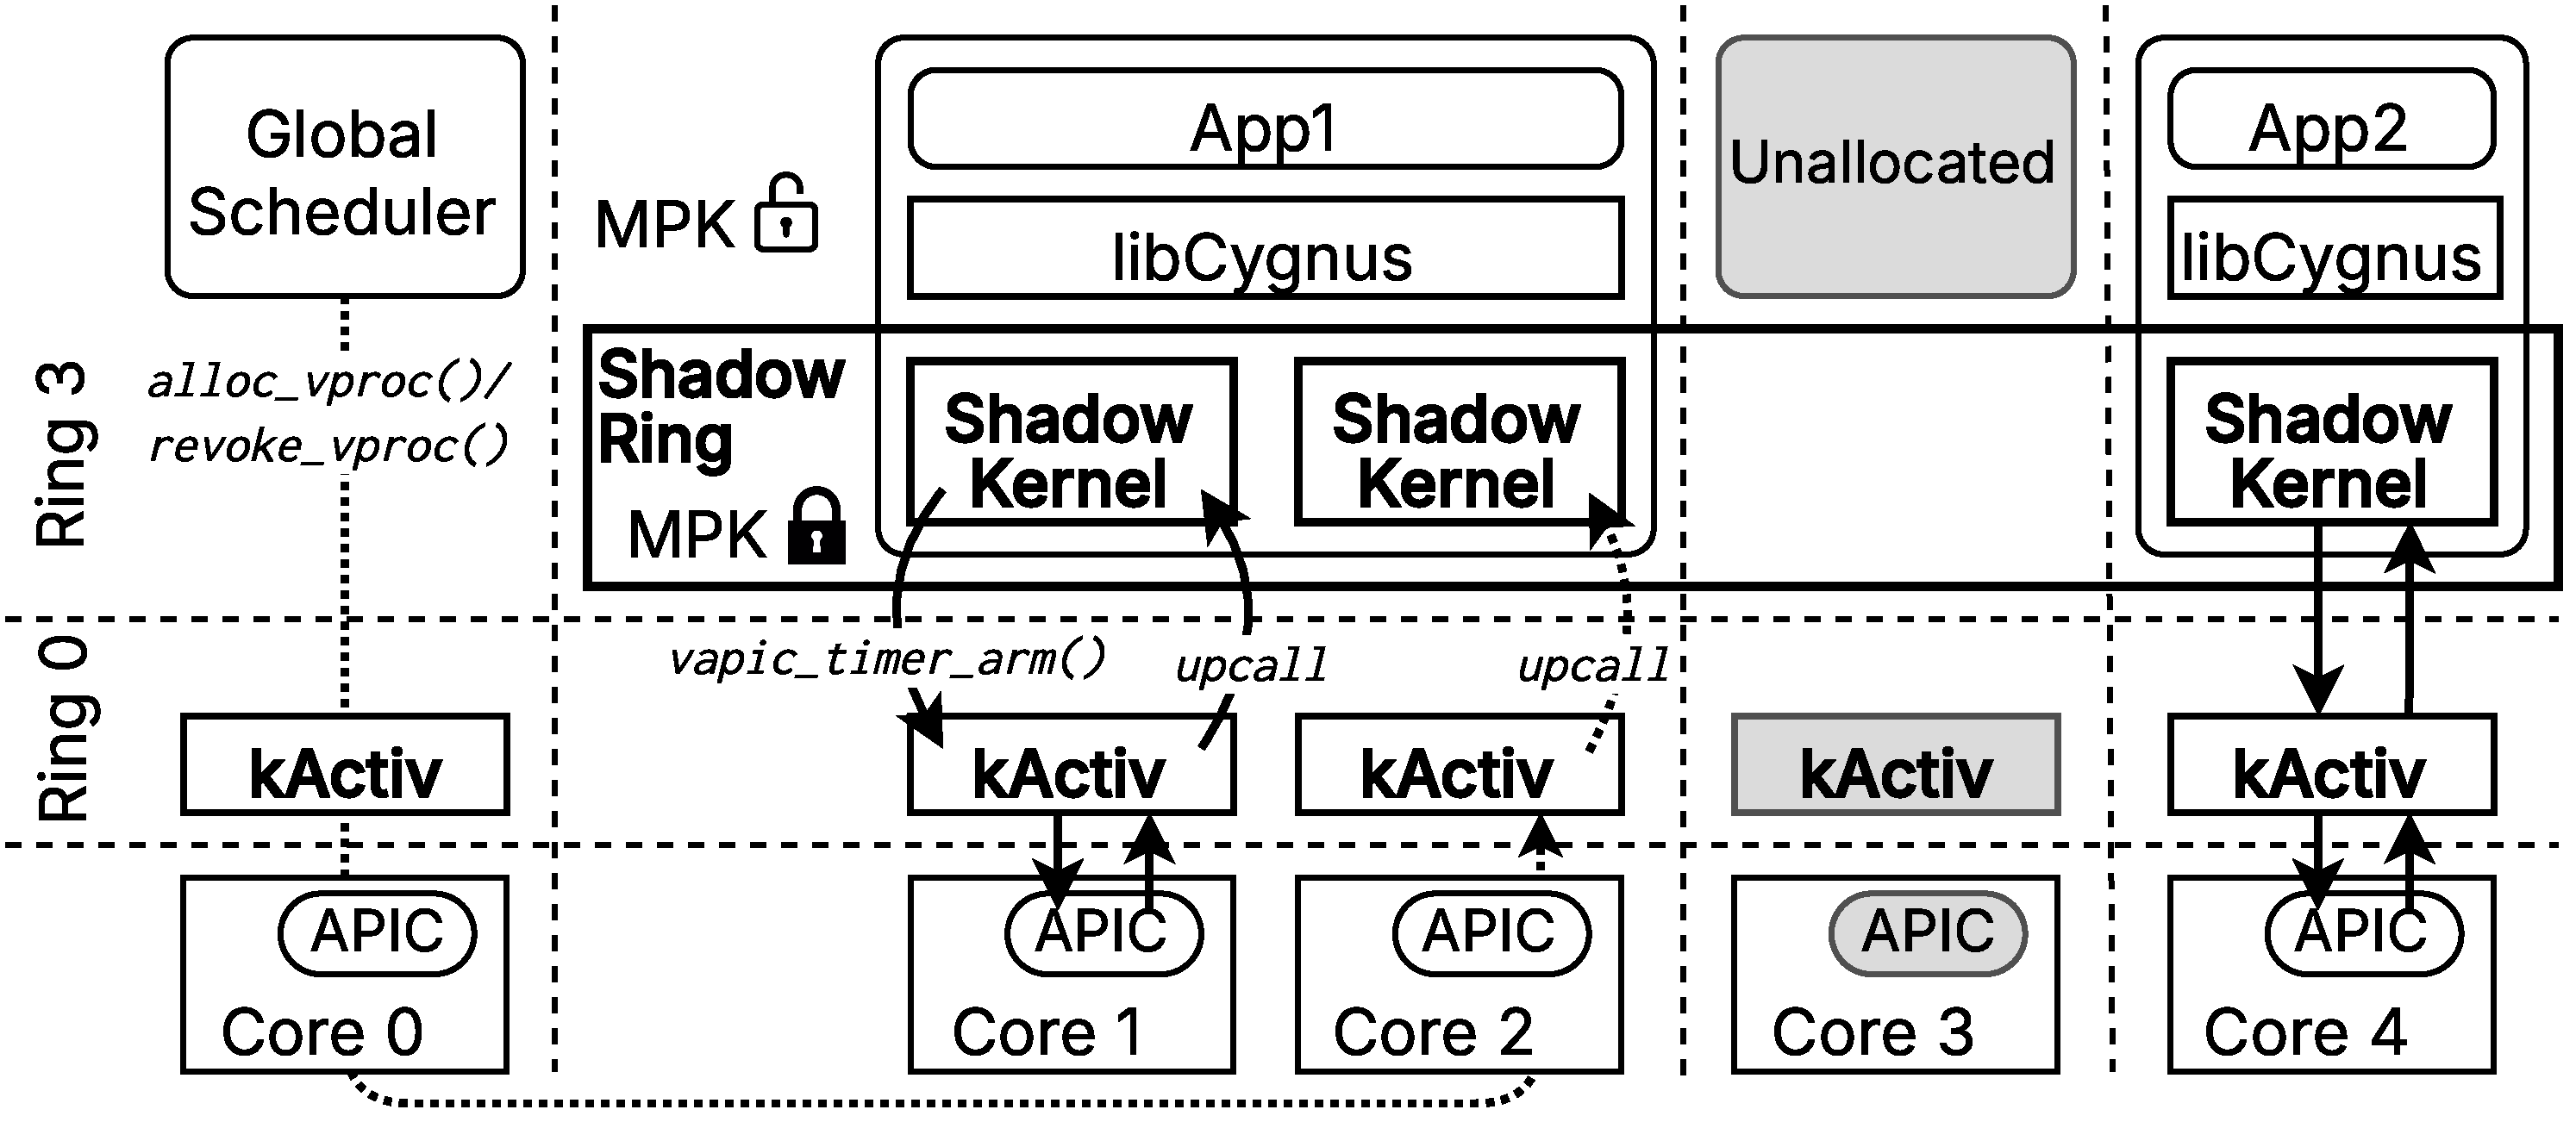
\includegraphics[width=\linewidth]{figs/overview.pdf}
    \label{fig:overview}
    \caption{\sysname Overview}
\end{figure}

1. Shadow Ring
2. Secure Upcall

\subsection{Shadow Ring}

\subsection{Secure Upcall}

\bibliographystyle{ACM-Reference-Format}
\bibliography{sample-base}

\end{document}
\endinput
%%
%% End of file `sample-sigconf-authordraft.tex'.
